\documentclass[conference]{IEEEtran}
\IEEEoverridecommandlockouts
\usepackage{cite}
\usepackage{cancel}
\usepackage{amsmath,amssymb,amsfonts}
\usepackage{algorithm}
\usepackage{algorithmicx}
\usepackage{algpseudocode}
\usepackage{siunitx}
\usepackage{graphicx}
\usepackage{float}
\usepackage{tikz}
\graphicspath{{images/}}
\usepackage{textcomp}
\def\BibTeX{{\rm B\kern-.05em{\sc i\kern-.025em b}\kern-.08em
    T\kern-.1667em\lower.7ex\hbox{E}\kern-.125emX}}
\begin{document}

\title{Segregation without Computation}

\author{\IEEEauthorblockN{Jordan Burklund}
\IEEEauthorblockA{\textit{Worcester Polytechnic Institute} \\
Worcester, MA \\
jsburklund@wpi.edu}
\and
\IEEEauthorblockN{Michael Giancola}
\IEEEauthorblockA{\textit{Worcester Polytechnic Institute} \\
Worcester, MA \\
mjgiancola@wpi.edu}
\and
\IEEEauthorblockN{Peter Mitrano}
\IEEEauthorblockA{\textit{Worcester Polytechnic Institute} \\
Worcester, MA \\
pdmitrano@wpi.edu}
}

\maketitle

\begin{abstract}
  In this paper, we demonstrate that memoryless computeless robots are capable of $n$-class segregation. We evolve controllers for this behavior with a genetic algorithm and perform a grid search over all parameters to understand the full parameter space. We find that robust segregation is possible, although not guaranteed. Instead, we prove that aggregation of kin robots is guaranteed when some reasonable conditions are met.
\end{abstract}

\begin{IEEEkeywords}
  swarm robotics, robot aggregation, robot segregation
\end{IEEEkeywords}

\section{Introduction and Related Work}

  Many prior methods have demonstrated the ability to aggregate robots and objects in a distributed way, and some have shown the ability to perform such tasks with limited computation and sensing capabilities. Decentralized aggregation is frequently posed as a precursor to other swarm behaviors such as sorting, self-assembly, or coordinated motion \cite{gauci_evolving_2014} \cite{dorigo_evolving_2004}. Segregation is a natural extension of aggregation, and so we also desire algorithms for segregating robots into different clusters. In order to make this robust to individual failures and simple to implement, we would also like to achieve segregation with no communication between robots, no complex sensors, no leaders or beacons, and no environmental cues.

  In nature, we find many examples of aggregation and segregation. Segregation occurs in cells during embryogenesis, and segregation of objects can be found in ants who sort their brood \cite{santos_segregation_2014}. Furthermore, segregation is something humans do very quickly, and we can do so almost on reaction rather than carefully planned motion. These examples motivate the study of simple controllers for segregation.

  \subsection{Aggregation and Segregation}
    Robot aggregation is defined as having all robots in the swarm collect at a particular location in a distributed manner. Many swarm aggregation policies require robots to compute bearing and distance to other robots, to sense gradients in the environment, or to otherwise communicate information. However, implementing these communication systems is difficult in practice, so methods that do not require communication or complex sensing are desirable. In \cite{gauci_self-organized_2014}, the authors propose a new class of policies that require no computation.

    The work of \cite{gasparri_swarm_2012} does not restrict itself to a computeless or memoryless solution. Instead they develop an aggregation algorithm which enables robots to respond to guidance commands -- i.e., a human using hand gestures to indicate which direction the swarm should move. They show that swarms running their algorithm are able to follow guidance commands and stay aggregated without colliding. A simpler controller is used in \cite{bahgeci_evolving_2005}, where robots are equipped with IR distance sensors surrounding the robot, 4 microphones, and an omni-directional speaker. The policy is a linear combination of the IR sensor values and the intensity values of the microphones. The authors show that a genetic algorithm is able to find weights for the policy such that robots aggregate together. In \cite{ando_distributed_1999}, the authors present a robot aggregation model with very limited sensing and no memory, but allows the robots to perform computations to determine their next position. They prove that their algorithm is correct in theory, then run the algorithm in simulation.

    Finally, \cite{gauci_self-organized_2014} considers only binary sensor that maps directly to wheel velocities. The authors demonstrate extremely robust aggregation despite these limitations, and they also prove formally that aggregation is guaranteed and find theoretical bounds on aggregation time in simple situations. Similarly, the authors of \cite{gauci_clustering_2014} perform object aggregation with the same restrictions on sensing and control.

    Segregation of robots has received little attention in swarm robotics, however many researchers have focused on sorting of objects \cite{vardy_accelerated_2012} \cite{holland_collective_1998} \cite{tao_wang_collective_2004} \cite{holland_stigmergy_1999}. The study in \cite{santos_segregation_2014} shares our objective, however they assume that each class has the same number of robots and that each robot knows the position of all other robots. In contrast, we adhere to the memoryless computeless controller architecture with a simple ternary sensor. \cite{gros_segregation_2009} also explores segregation robots based on local interactions inspired by gravity, however they require a centralized broadcast or a consensus algorithm to agree on the source or direction of gravity.

  \subsection{Robots That Do Not Compute}

    The memoryless and computeless controllers originally proposed by \cite{gauci_self-organized_2014} has been extended to other tasks and been modified in many ways by other researchers.

    In \cite{kernbach_re-embodiment_2009}, the authors propose an aggregation policy roughly based on observations of bees clustering in an optimal temperature location. In their method, robots are only able to distinguish between collisions between another robot or a wall, can only sense the intensity of a light source when they have collided, and do not communicate information. Although the robots have limited sensing and communication capabilities, the authors show that robots can aggregate to an optimal light intensity location, and that the time to converge to the optimal location improves with increasing number of robots in the environment.

    Robots that do not compute and are memoryless have also been shown to aggregate around a specific object, circle in a ring around an object, and forage for obstacles \cite{johnson_evolving_2016}. In this work, the authors show one can construct simple cost functions to guide the evolution of controllers to do new yet interesting tasks. However, they also report that in attempting to evolve a controller to rendezvous the robots around an object, they accidentally and consistently evolved a policy where the robots circled around the target object. This demonstrates that designing a cost function can be hard or unreliable. They achieved rendezvous by initializing the policy at generation zero to the policy found in \cite{gauci_self-organized_2014} for simple aggregation.

\section{Methodology}

  \subsection{Problem Formulation}

    We consider a collection of differential drive robots all executing the same controller in a homogeneous, two dimensional, obstacle free environment. The robots are equipped with a single forward facing line of sight sensor which can distinguish between the presence of a kin robot, a non-kin robot, and nothing. This sensor is assumed to have infinite length (we consider non-infinite length in Section \ref{section:beam_length}). We assign $I=0$ to the state when no robot is seen, $I=1$ to the detection of a kin robot, and $I=2$ to the detection of a non-kin robot. We allow for any number of classes, but the robots need not distinguish between different non-kin classes. They need only to detect if a robot is of the same class or not. The objective is to segregate robots into clusters, ideally such that all the robots of the same class are packed into one cluster with no non-kin robots.

    \begin{algorithm}[t!]
      \begin{algorithmic}
      \If {$I=0$} \State set wheel speeds to $v_{l_0}$, $v_{r_0}$
      \ElsIf {$I=1$} \State set wheel speeds to $v_{l_1}$, $v_{r_1}$
      \Else \State set wheel speeds to $v_{l_2}$, $v_{r_2}$
      \EndIf
      \end{algorithmic}
      \caption{The structure of the controller}
      \label{alg:controller}
    \end{algorithm}

    The controllers we use in our experiments are of the same form as in \cite{gauci_self-organized_2014}. They simply map each of the three sensor values to a set of wheel speeds. Psuedo code for the controller is shown in Algorithm \ref{alg:controller}. This controller has six parameters:

    $$[\,v_{l_0}, v_{r_0}, v_{l_1}, v_{r_1}, v_{l_2}, v_{r_2}\,]$$

    Keeping with the form used in \cite{gauci_self-organized_2014}, we let these parameters range from -1 to 1. In simulation, we then scale this parameter to range from \SI{-20}{\centi\meter\per\second} to \SI{20}{\centi\meter\per\second}. We now describe two approaches for finding these parameters, genetic algorithms and grid search.

  \subsection{Simulation Environment}

    We use the ARGoS simulation environment to search for controller parameters and evaluate them, which has the advantage of allowing us to run trials much faster than on real robots \cite{pinciroli_argos:_2012}. In our simulations, we use a range and bearing sensor to implement the theoretical line of sight sensor. Specifically, we consider all of the robots within some imaginary beam angle and pick the closest of those. In our analysis, we describe the sensor as infinitely thin, but in practice it must have some small finite angle. We explore the performance effect of various beam angles in Section \ref{section:beam_angle}.

  \subsection{Evolving Segregation}

    In order to quickly search for parameters to achieve segregation, we use a simple genetic algorithm to evolve controller parameters. The genetic algorithm we used is unmodified from the example MPGA code provided with the ARGoS simulator. The mutation strategy is simply to mutate each of these 6 parameters with some probability p ($0.05$ in our experiments). If a parameter is selected to be mutated, a uniformly random number from -1 to 1 is picked for the new value. Selection is performed by picking the two lowest cost individuals, and the next population is formed by crossing the parameters of these two individuals. The original two parents are always kept in the population so that the current lowest cost individual is never removed until a lower cost genome is discovered.

  \subsection{Cost Functions}

    As with any optimization algorithm, it is important to have a cost function that accurately assigns cost to behaviors. We explore two different cost functions, and we find that while both of them are intuitive they did not behave as we expected (see Section \ref{section:evaluting_cost_functions}). The first is the cluster metric used by \cite{gauci_self-organized_2014}, which is the proportion of the number of robots in the largest cluster to the total number of robots. We will apply this for each class of robots and sum up the cluster-metric cost for each class to get the total cost. The negative sign is present because the cluster metric is 0 when no robots are connected and 1 when all robots in a class are connected, so the negative sign makes mores connections a lower cost. This was ultimately the cost function we used in all of our experiments.

    \begin{align*}
      c_{\text{total}} &=  \sum_{\text{classes}}\sum_{t=0}^{T-1} -t c_{\text{gauci}}^{(t)} \\
    \end{align*}

    We also tried a new cost function to address some concerns with the cluster metric. The cluster metric described above is problematic because it considers a straight line of robots to be one cluster. In some scenarios, we care about how tightly the swarm is packed in its clusters. This new metric uses the centroids of the robots in each class. We borrow the dispersion metric $u^{(t)}$ from \cite{gauci_self-organized_2014}, which essentially computes the sum of distances from each robot to the centroid, but in our case we apply this to each class of robots. Consider $u_i^{(t)}$ to be the dispersion of a particular class $i$ at time $t$. Given all the centroids $\bar{p}_i^{(t)}$ for each class $i$, we call the centroid of all of these centroids $\bar{P}^{(t)}$. We call this the centroid-of-centroids cost function, and it can be defined formally as follows:

    \begin{align*}
    c_{\text{intra}} &= \sum_{i=1}^n u_i^{(t)} \\
    c_{\text{inter}} &= -\frac{1} {4r^2}\sum_{i=1}^n{\lVert \bar{p}_i^{(t)} - \bar{P}_i^{(t)} \rVert}^2 \\
    c_{\text{total}} &=  \sum_{t=0}^{T-1} t (c_{\text{intra}} + c_{\text{inter}}) \\
    \end{align*}

  \subsection{Grid Search}

    In order to exhaustively search the space of possible controllers, we conduct a grid search of the 6-dimensional parameter space. Due to limited computational resources, we were only able to search with a resolution of 7 values per parameter, which means in total we evaluated $7^6=117649$ parameters. For each parameter, we ran 1 trial in 36 different initial configurations, with 180 seconds for each simulation. These configurations consisted of uniformly random placement, clusters, and lines of robots distributed throughout the environment. We chose to include some structure configurations (clusters and lines) because we discovered that they varied significantly in performance from uniform random configurations, and by explicitly evaluating on structure configurations we can speak more confidently about the ability of the controller to succeed in any configuration. Otherwise, we would need to have far more trials with uniformly random robot placement to make the same claims. We were able to parallelize across the 36 configurations and run at 75x real time, so the entire grid search took approximately 4 days to evaluate all the controllers.

    Because the search space is 6 dimensional, we choose to visualize it by plotting every pair of parameters against each other. For example, we consider how the cost changes as $v_{l_0}$ and $v_{r_0}$ change. We note that these graphs, shown in Figure \ref{fig:grid_search}, show very similar patterns to the same plots presented by \cite{gauci_self-organized_2014}. As an example of readding these plots, we can tell from plot of parameters 2 and 3 ($I=1$) that there were no good controllers where the left and right wheel speeds were equal and negative since there are only dark square in the upper left, and that the best controllers had slightly unequal but close to 1 because the bottom left squares are lightest. These plots also visualize how there are some sharp discontinuities where performance changes dramatically.

    \begin{figure}
      \centering
      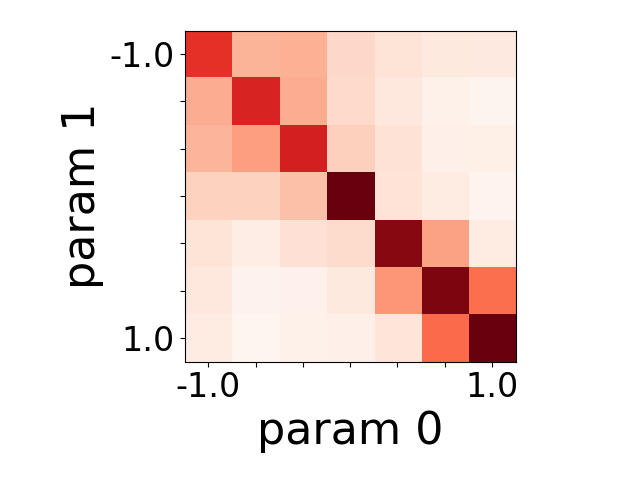
\includegraphics[width=0.42\linewidth]{./images/0_1_grid_img.png}
      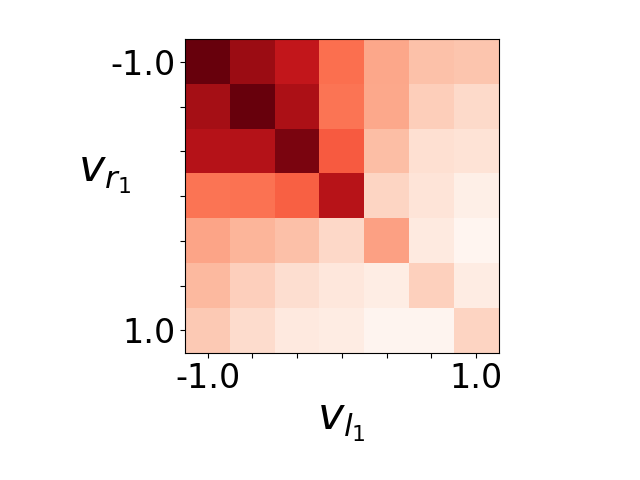
\includegraphics[width=0.42\linewidth]{./images/2_3_grid_img.png}
      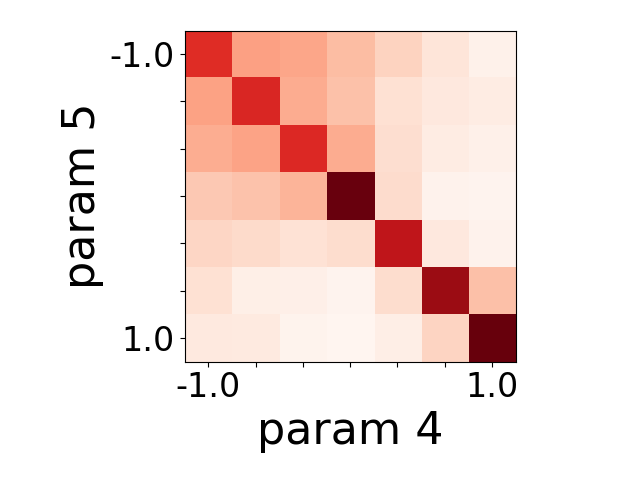
\includegraphics[width=0.42\linewidth]{./images/4_5_grid_img.png}
      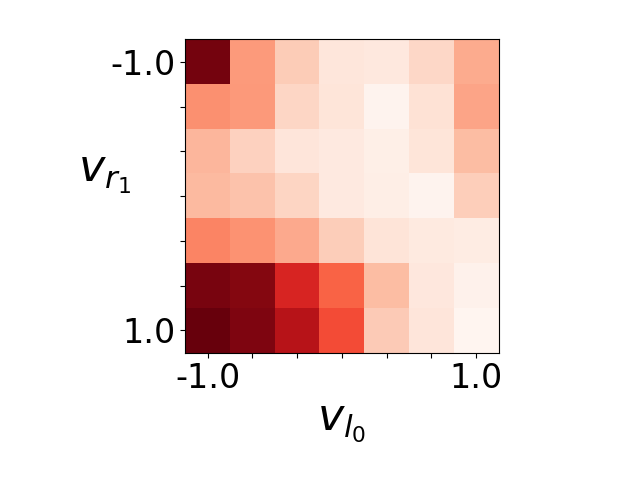
\includegraphics[width=0.42\linewidth]{./images/0_3_grid_img.png}
      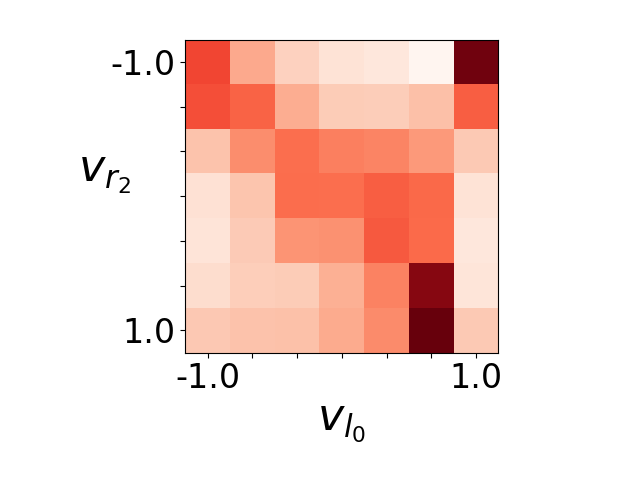
\includegraphics[width=0.42\linewidth]{./images/0_5_grid_img.png}
      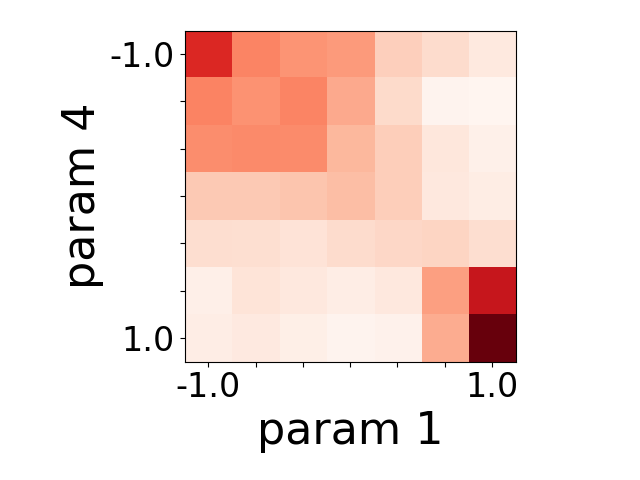
\includegraphics[width=0.42\linewidth]{./images/1_4_grid_img.png}
      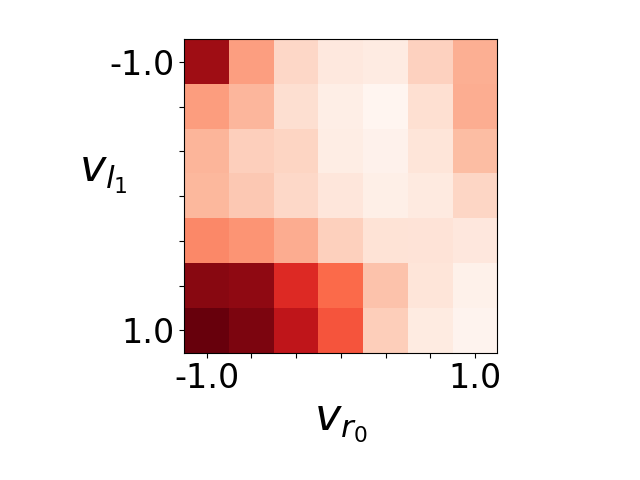
\includegraphics[width=0.42\linewidth]{./images/1_2_grid_img.png}
      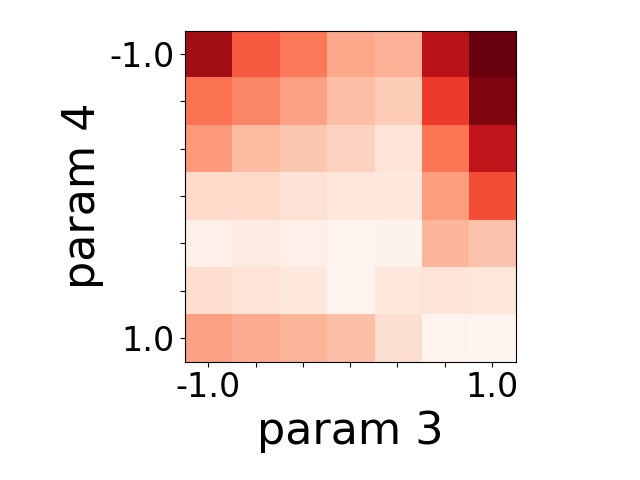
\includegraphics[width=0.42\linewidth]{./images/3_4_grid_img.png}
      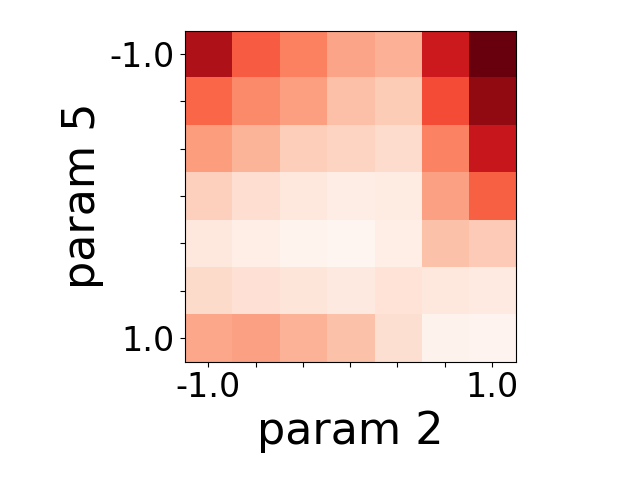
\includegraphics[width=0.42\linewidth]{./images/2_5_grid_img.png}
      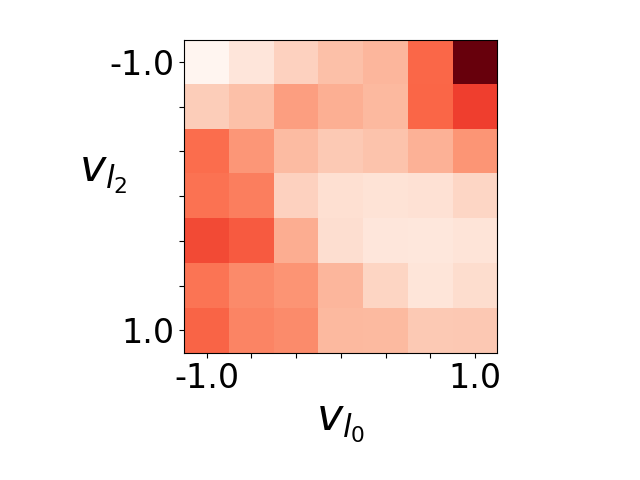
\includegraphics[width=0.42\linewidth]{./images/0_4_grid_img.png}
      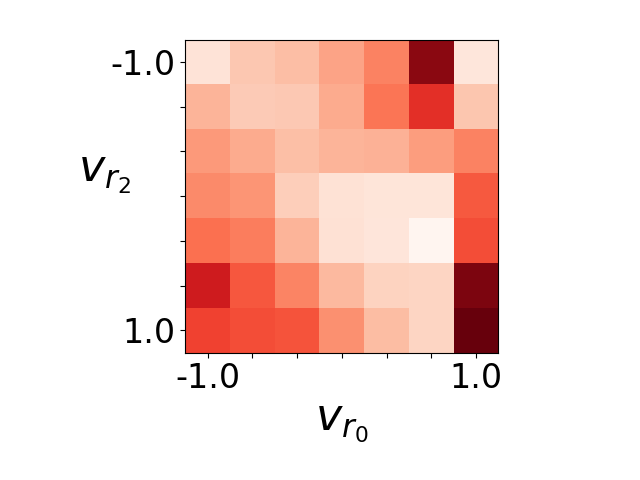
\includegraphics[width=0.42\linewidth]{./images/1_5_grid_img.png}
      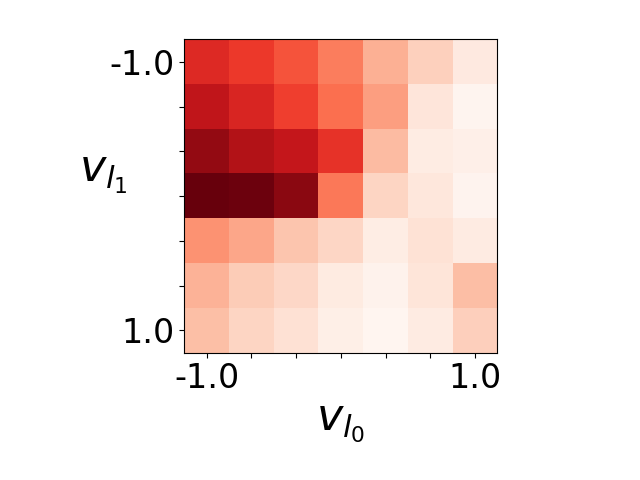
\includegraphics[width=0.42\linewidth]{./images/0_2_grid_img.png}
      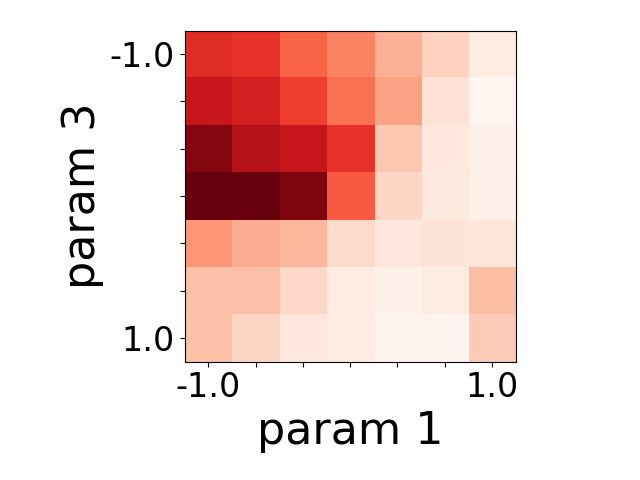
\includegraphics[width=0.42\linewidth]{./images/1_3_grid_img.png}
      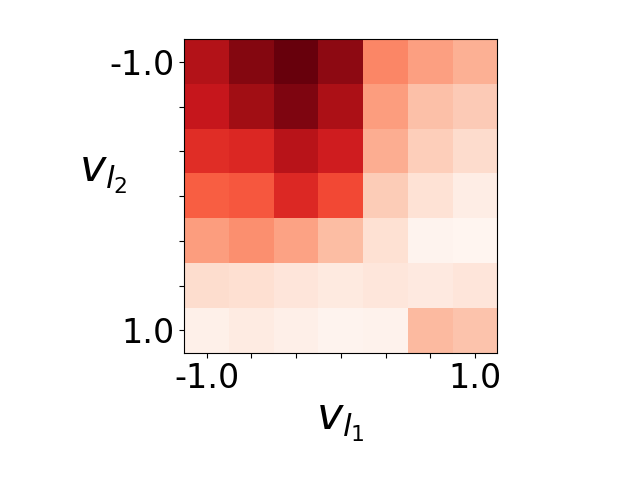
\includegraphics[width=0.42\linewidth]{./images/2_4_grid_img.png}
      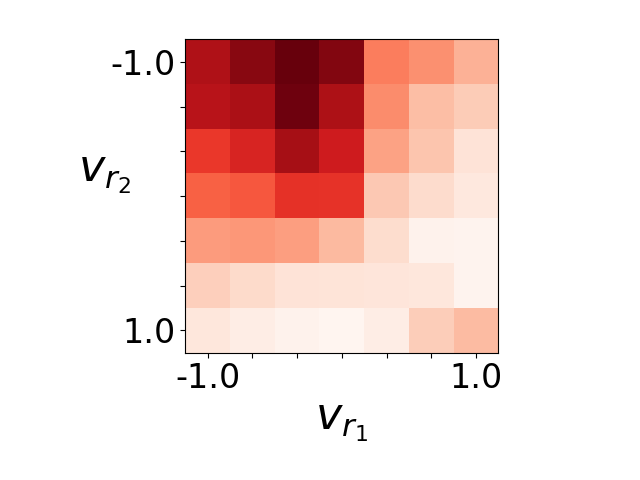
\includegraphics[width=0.42\linewidth]{./images/3_5_grid_img.png}
      \caption{Each grid cell shows the cost of the best controller with the x-axis and y-axis parameters at that given cell value.}
      \label{fig:grid_search}
    \end{figure}

\section{Controller Analysis}

  \subsection{Aggregation with static Kin}

    Using a grid search we found imperially that the parameters [1, -0.6667, 0.3333, 1.0, 1.0, 0.0] best achieve segregation as defined by our cluster metric cost function. We now analyze this controller formally. First, we prove that a single isolated robot executing this controller will aggregate to a static kin robot, or more importantly, a static cluster of kin robots. This proof is a variation of the Theorem 5.1 provided in \cite{gauci_self-organized_2014}. Consider a robot situated as shown in Figure \ref{fig:kin_aggregation}. The controller dictates that since a kin robot is seen, $I=1$, so $v_{l_1} = 0.3333$ and $v_{r_1} = 1$. This will cause the robot to turn counter-clockwise with some radius $R$. Without loss of generality, we define our coordinate system so that $c_i=[0,0]$ with the robot $i$ facing the $+x$ axis. For this analysis, we assume that the robot has a fixed, positive inter wheel distance $W$, and that the controller is executed in finite time steps. Our goal is to show that the distance between the position of the robot after executing our controller for one time step $p'_i$ and the kin robot $p_j$ is less than the distance between the initial position of the robot $p_i$ and the kin robot $p_j$. Formally, this is expressed by the following relationship:

    \begin{equation} \label{eq:agg}
      \lVert p_j - p'_i \rVert < \lVert p_j - p_i \rVert
    \end{equation}

    \begin{figure}
      \centering
      \begin{tikzpicture}
        \draw[white] (-2.25,3.5) rectangle(7,-4.75);

        \draw[->] (0,0) -- (6,0);
        \node at (6.2,.2) {x};
        \draw[->] (0,0) -- (0,3);
        \node at (-0.2,3.2) {y};

         % c_i
        \filldraw (0,0) circle (.05);
        \node at (.2,.2) {$c_i$};
        \draw[blue, dashed] (0,0) circle (2);

         % p_i
        \filldraw (0,-2) circle (.05);
        \node at (.2,-2.2) {$p_i$};
        \draw[blue] (0,-2) circle (0.85);
        \node at (-.3,-.8) {$R$};
        \draw[dashed] (0,0) -- (0,-2);

         % p'_i
        \filldraw (1.41,-1.41) circle (.05);
        \node at (1.85,-1.25) {$p'_i$};
        \draw[blue] (1.41,-1.41) circle (0.85);
        \draw[dashed] (0,0) -- (1.41,-1.41);
        \node at (.8,-.3) {$R$};

         % p_j
        \filldraw (5,-3.25) circle (.05);
        \node at (5.2,-3.5) {$p_j$};
        \draw[red] (5,-3.25) circle (1.25);
        \draw (5,-3.25) -- (5,-2);
        \node at (5.3,-2.625) {$r_j$};

        % delta
        \draw[blue] (0,-2) -- (5,-2);
        \draw[blue] (1.41,-1.41) -- (5.3,-2.03);
        \node at (2.5, -2.2) {$\delta$};

        % theta
        \draw (0,-.7) arc [radius=.7, start angle=-90, end angle=-45];
        \node at (.36,-.85) {$\theta$};
      \end{tikzpicture}
      \caption{The robot will always move closer to its Kin.}
      \label{fig:kin_aggregation}
    \end{figure}


    We emphasize that $r_j$ could be the radius of a single kin robot or the radius of a large cluster of kin robots. With this coordinate system defined and assumptions stated, we can define the coordinate of $p_i$, $p_j$, and $p'_i$.

    \begin{equation}
      \begin{split}
        p_i = \begin{bmatrix}0 \\ -R\end{bmatrix} \\
        p_j = \begin{bmatrix}\delta \\ -(R+r_j)\end{bmatrix} \\
        p'_i = \begin{bmatrix}R\sin(\theta) \\ -R\cos(\theta)\end{bmatrix}
      \end{split}
    \end{equation}

    We then substitute these variables into our inequality (Equation \ref{eq:agg}), and the result is shown in Equation \ref{eq:agg_result}. For the full derivation, see Appendix \ref{thm:1}. In short, the distance of the robot to its kin is guaranteed to decrease until a point where the sensor ray distance $\delta$ is not greater than some simple function of $\theta$ and $R$.

    \begin{equation} \label{eq:agg_result}
      \delta > (R + r_j)\tan\bigg(\frac{\theta}{2}\bigg)
    \end{equation}

    We can further calculate exactly how much closer the robot $i$ will be to robot $j$ after executing the $I=1$ state for one time step. As we show in Appendix \ref{thm:2}, the change in distance between the robots is exactly equal to Equation \ref{eq:dist_change}. We can use this equation to plot how the distance between the robots changes over time. We show an example of this for our simulated robot in Figure \ref{fig:dist_plot}.
    \begin{equation} \label{eq:dist_change}
      2R\big((r_j + R)(1 - \cos(\theta))-\delta\sin(\theta)\big)
    \end{equation}

    In both of these equations the dependant variables $\theta$ and $R$ are themselves a function of $\Delta t$, the inter wheel diameter $W$, and the wheels speeds of the controller $v_{l_1}$ and $v_{r_1}$, which are shown in Equation \ref{eq:theta_and_r}.

    \begin{align}
      \begin{split} \label{eq:theta_and_r}
        \theta &= \Delta t\omega = \Delta t \frac{v_{r_1} - v_{l_1}}{W} = \Delta t \frac{1 - (0.3333)}{W} = \frac{2\Delta t}{3W} \\
        R &= \frac{W}{2}\bigg(\frac{v_{r_1} + v_{l_1}}{v_{r_1} - v_{l_1}}\bigg) = \frac{W}{2}\bigg(\frac{1 + (0.3333)}{1 - (0.3333)}\bigg) = \frac{W}{4}
      \end{split}
    \end{align}

    Combining \ref{eq:theta_and_r} with \ref{eq:agg_result} gives us \ref{eq:agg_final_result}, which tells us the conditions under which aggregation is guaranteed. We emphasize that this does not mean aggregation to a kin is guaranteed for all values of $\Delta t$, $r_j$, and $W$. For example, if $\Delta t$ is increased to \SI{1}{\second} then aggregation is likely not guaranteed, simply because robot $i$ will have driven very far in its arc in that time.

    \begin{figure}
      \centering
      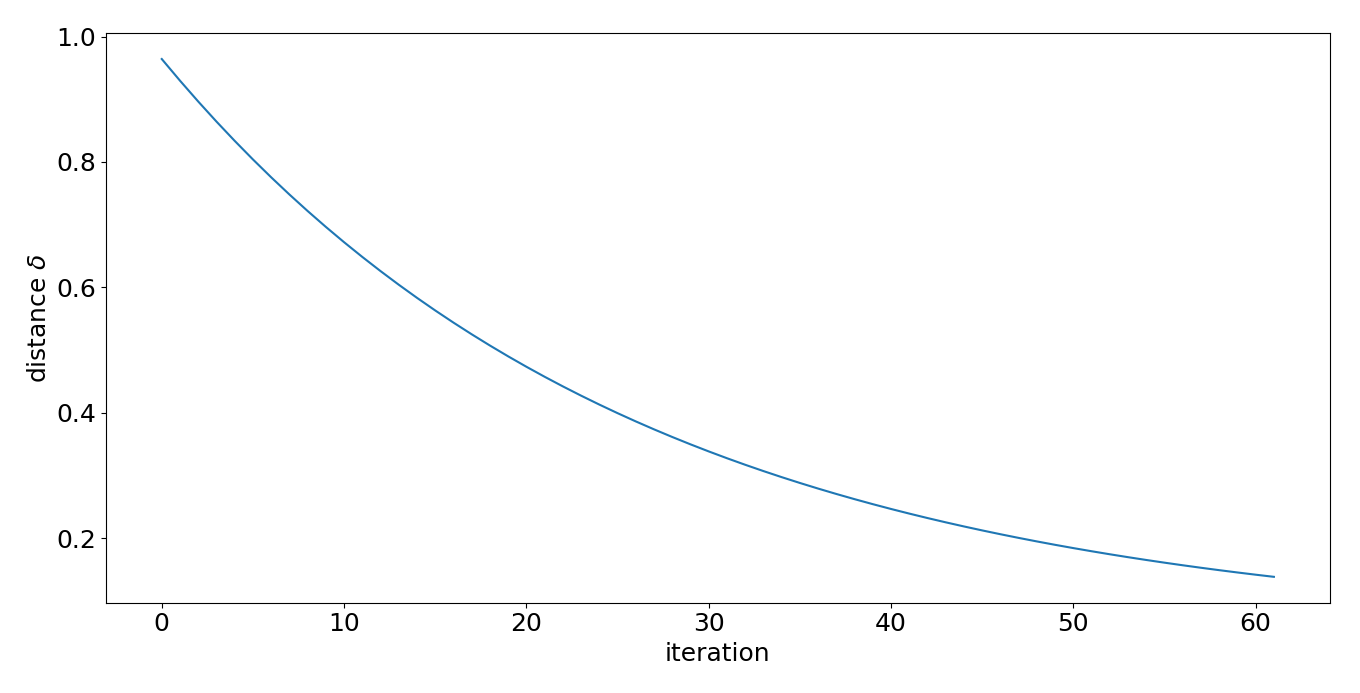
\includegraphics[width=1\linewidth]{./images/dist_plot.png}
      \caption{The distance between a robot and its kin after each step as it aggregates. We use $W=0.14$, $r_j=0.14$, $\Delta t=0.1$. In this example, aggregation took 60 iterations.}
      \label{fig:dist_plot}
    \end{figure}

    \begin{equation}
      \label{eq:agg_final_result}
      \delta > \bigg(\frac{W}{4} + r_j\bigg)\tan\bigg(\frac{\Delta t}{3W}\bigg)
    \end{equation}

    We can now consider an example with the Khephera IV robot. The inner wheel distance for the Khephera IV is $W=0.14$m, and in our simulations we use a time step of $\Delta t = 0.1s$. Therefore $\theta = 0.4761\;\text{rad}$ and $R=0.035$, and so aggregation is guaranteed when the following is true.

    \begin{equation} \label{eq:khephera_agg}
      \begin{split}
        \delta &> \bigg(0.035 + r_j\bigg)\tan\frac{0.4761}{2} \\
        \delta &> 0.2427 r_j + 0.0085
      \end{split}
    \end{equation}

     What we would like is for the right hand side of the equation to always be less than the distance at which the robots are considered aggregated. In other words, we want aggregation to be guaranteed until the sensor ray distance is small enough that aggregation has been achieved. We defined aggregation as when the distance between the robots $d \leq r_j+r_i$. Since the sensor ray length $\delta$ is always less than that distance, we can simply show that the right hand side of Equation \ref{eq:agg_final_result} is always less than $r_i+r_j$. Again we must consider an example since aggregation cannot be guaranteed in all scenarios, so going back to our example with the Khephera IV, we note that $0.2427r_j + 0.0085 < r_i+r_j$ is always true because both $r_j$ and $r_i$ must be positive.

     We examined a wide range of possible values for our parameters $\Delta t$, $r_i$, $W$, and $r_j$, and we find that as long as $\Delta t$ is small (less than 0.25s), then aggregation is guaranteed for reasonable values of the other parameters (less than 0.5m).

  \subsection{Aggregation with non-static Kin}

    \begin{figure}[H]
      \centering
      \begin{tikzpicture}
        \draw[white] (-2.25,3.5) rectangle(7,-4.75);

        \draw[->] (0,0) -- (6,0);
        \node at (6.2,.2) {x};
        \draw[->] (0,0) -- (0,2);
        \node at (-0.2,2.2) {y};

         % c_i
        \filldraw (0,0) circle (.05);
        \node at (.2,.2) {$c_i$};

         % c_j
        \filldraw (5,-4.75) circle (.05);
        \node at (5.2,-4.95) {$c_j$};

         % p_i
        \filldraw (0,-2) circle (.05);
        \node at (.2,-2.2) {$p_i$};
        \draw[blue] (0,-2) circle (1);
        \node at (-.3,-.8) {$R$};
        \draw (0,-2) -- (-0.7071,-1.29);
        \node at (-0.4,-1.9) {$r_i$};
        \draw[dashed] (0,0) -- (0,-2);

         % p'_i
        \filldraw (1.41,-1.41) circle (.05);
        \node at (1.85,-1.25) {$p'_i$};
        \draw[blue] (1.41,-1.41) circle (1);
        \draw[dashed] (0,0) -- (1.41,-1.41);
        \node at (.8,-.3) {$R$};

         % p_j
        \filldraw (5,-2.75) circle (.05);
        \node at (5.25,-3.0) {$p_j$};
        \draw[red] (5,-2.75) circle (0.75);
        \draw (2,-2.75) arc [radius=.7, start angle=180, end angle=192];
        \draw (1.95,-2.80) -- (1.8,-3.35);
        \draw[dashed] (5,-2.75) -- (0,-2.75);
        \node at (1.8,-3.5) {$\alpha$};
        \draw[red] (5,-2.75) -- (0,-3.00);
        \draw (5,-2.75) -- (5.53,-2.21);
        \node at (5.15,-2.3) {$r_j$};
        \draw[dashed] (5,-2.75) -- (5,-4.75);

         % p'_j
        \filldraw (3.59,-3.34) circle (.05);
        \node at (3.39,-3.69) {$p'_j$};
        \draw[red] (3.59,-3.34) circle (0.75);
        \draw[dashed] (3.59,-3.34) -- (5,-4.75);

        % delta
        \draw[blue] (0,-2) -- (5,-2);
        \node at (2.5, -2.2) {$\delta$};

        % theta
        \draw (0,-.7) arc [radius=.7, start angle=-90, end angle=-45];
        \node at (.36,-.85) {$\theta$};
      \end{tikzpicture}
      \caption{The generic scenario of two robots executing the segregation controllers. In our proof, we allow for robots to be different sizes.}
      \label{fig:pair_kin_aggregation}
    \end{figure}

    We extend the proof above to consider the case of two kin robots executing the controller. In Figure \ref{fig:pair_kin_aggregation}, we see the situation where two kin robots are executing our controller. To justify that this as our starting state, we consider the three possible initial situations. If no robots see each other, they will both rotate until one or both detect the other. If one of the robots see its kin first, we find ourselves in the situation depicted. In this scenario, robot $i$ is in state $I=1$ and will arc to the left. If robot $j$ does not yet see robot $i$, it will continue to rotate until some time $t_b$ it does, otherwise it will simply keep rotating in state $I=0$. The final scenario where both robots see each other is a special case where $t_b=0$. In the case where robot $j$ doesn't sees robot $i$ until after $i$ finishes its arc away, we simply need to extend the proof from the static robot. We need now have to consider the point $p'_j$, which here refers to the position of robot $j$ after executing the tight arc of state $I=0$ for one time step. What we want to show, similarly to the earlier proof, is that the robots are closer after executing their moves than before. This is expressed formally is:

    $$\lVert p'_j - p'_i \rVert < \lVert p_j - p_i \rVert $$

\section{Experimental Results}

  \subsection{Evaluating the centroid-of-centroids cost function} \label{section:evaluting_cost_functions}

    When we implemented the centroid-of-centroids style cost function, we quickly found examples of configurations ranked in ways we did not like. One example is shown below in Figure \ref{fig:cost_function_fuckup}. The behavior that looks like aggregation was given lower cost of -8e9, versus the behavior that looks like segregation was given a cost of -5e9.

    \begin{figure}[H]
      \centering
      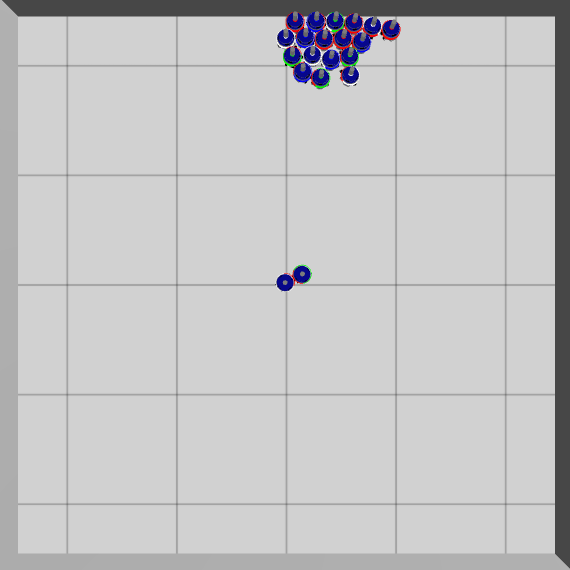
\includegraphics[width=0.49\linewidth]{./images/individual_0_gen_0.png}
      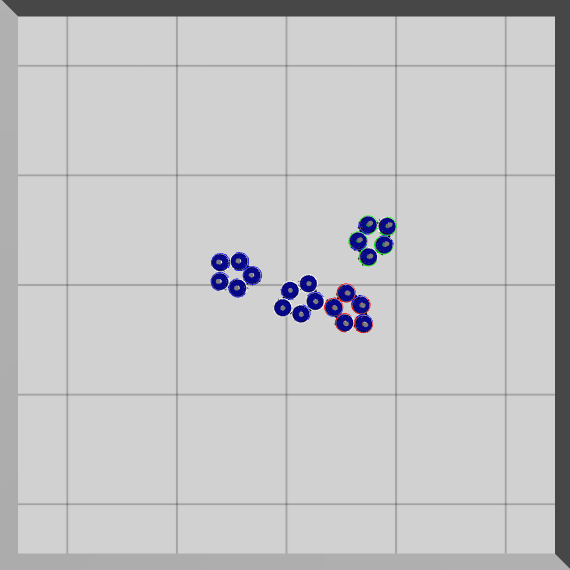
\includegraphics[width=0.49\linewidth]{./images/individual_0_gen_1_better.png}
      \caption{The left picture was given lower cost than the right, which is not desirable.}
      \label{fig:cost_function_fuckup}
    \end{figure}

  \subsection{The effect of Beam Angle} \label{section:beam_angle}

    In practice, there must be some finite beam angle to the theoretically line of sight sensor. We ran 100 trials in simulation with uniformly random initial distributions of 40 robots with various half beam angles. Figure \ref{fig:beam_angle} shows the results, as well as a diagram showing how we define half beam angle. The best half beam angle we tested was \ang{15}, and angles smaller or larger got progressively worse. We found that at lower beam angles, it was possible for a robot to skip over seeing a robot during a single step of turning. At larger angles, we believe the behavior fails because we choose the closest robot within the angle, so if a kin robots and non-kin robot are both visible but the non-kin robot is closer, it will execute the non-kin behavior and turn away from the kin robot, thus not aggregating to it.

    \begin{figure}[H]
      \centering
      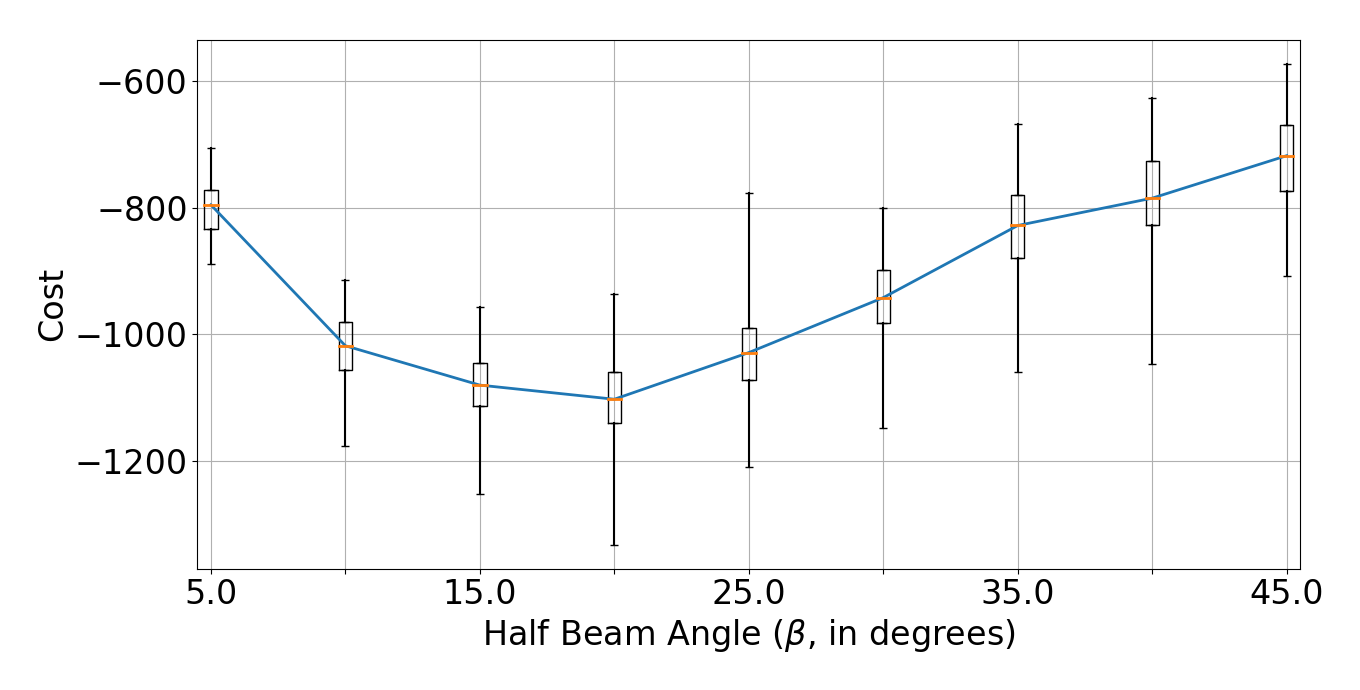
\includegraphics[width=1\linewidth]{./images/beam_angle.png}
      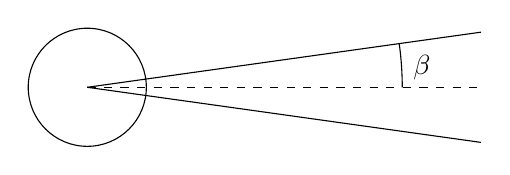
\begin{tikzpicture}
        \draw (0,0) circle (0.75);
        \draw (0,0) -- (5,0.7);
        \draw[dashed] (0,0) -- (5,0);
        \draw (0,0) -- (5,-0.7);
        \draw (4,0) arc [radius=4, start angle=0, end angle=8];
        \node at (4.25,0.25) {$\beta$};
      \end{tikzpicture}
      \caption{A \ang{15} degree half beam angle is best for segregation. Lower cost is better.}
      \label{fig:beam_angle}
    \end{figure}

  \subsection{The effect of Beam Length} \label{section:beam_length}

    We also consider what happens if our theoretically infinite sensor now has finite range. We use \ang{15} half beam angle and the same experimental setup as with the beam angle experiments. Like in \cite{gauci_self-organized_2014}, we consider the maximum range of the sensor as the diagonal length of the square in which the robot are initially distributed. In all our experiments, this box was \SI{5}{\meter\square}, so we consider a range of \SI{7.07}{\meter} to be effectively unlimited. We report the costs for beam lengths as a fraction of this maximum range. As you can see in Figure \ref{fig:beam_length}, in practice a beam length of only 35\% of the theoretical maximum performs just as well. Below this, the performance degrades. However, even a beam length of just 7\% of unlimited is more effective than zero length at segregation. In our experiment watching many simulations, beam length should also be scaled with the total number of robots as well as the initial distance between robots. When the beam length is short, there are many cases where two rings of kin robots form at different points in the environment, and in order for these two rings to join the robots must have sufficiently long beam length in order to detect each other.

    \begin{figure}
      \centering
      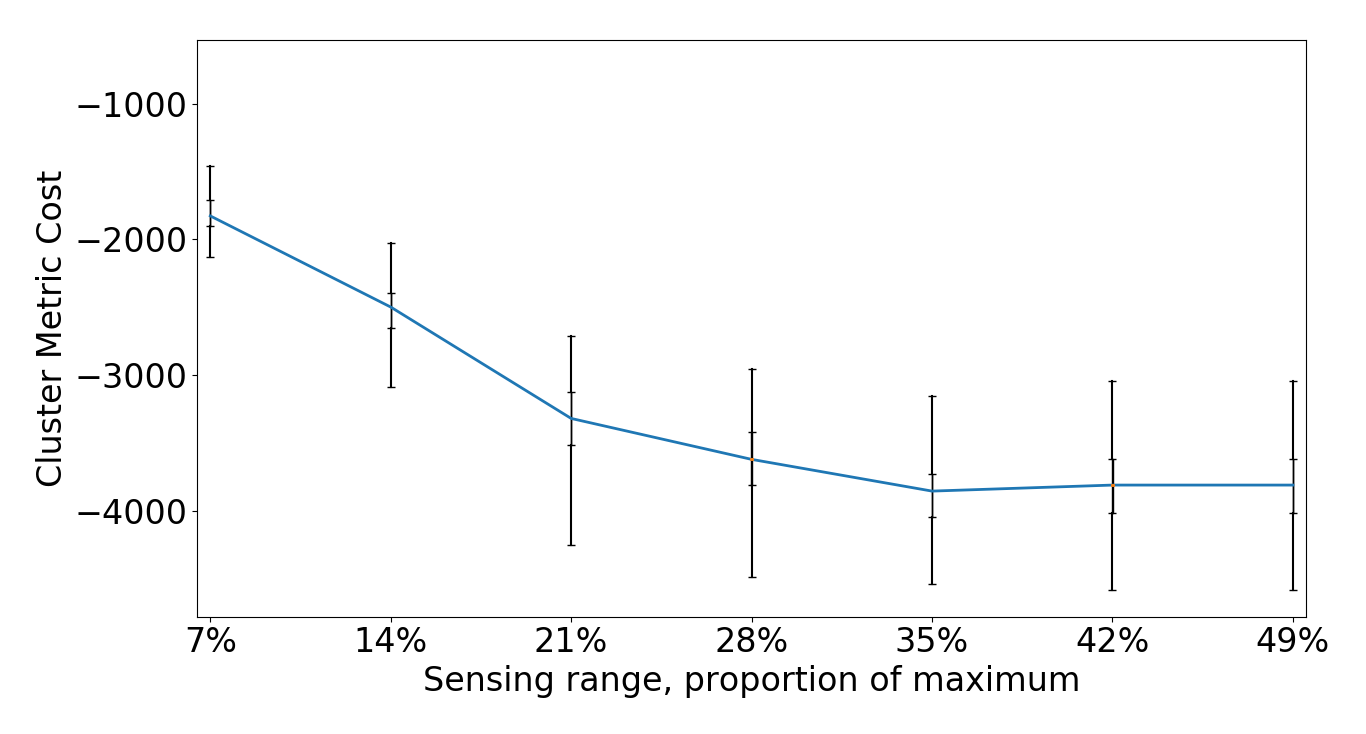
\includegraphics[width=1\linewidth]{./images/beam_length.png}
      \caption{Segregation is robust to very finite sensor beam lengths. The blue bar indicates the worst (highest) attainable cost in which all robots are isolated from any kin.}
      \label{fig:beam_length}
    \end{figure}

\section{Future Work}
An interesting expansion of this work would be to investigate more realistic applications i.e. different types of robots that need to segregate based on their type e.g. drones, footbots, etc. Since different types of robots will have different movement mechanisms, a single controller for all robots is likely to be inadequate. However, it is possible that there are similar computeless solutions.

%  - consider the radius of the robot, track width, etc...

\section{Conclusion}
In this paper, we demonstrate that memoryless, computeless robots are capable of $n$-class segregation. We use a simple controller design consisting of a 6-tuple; wheel speeds if a robot's line of sight sensor sees nothing, a robot of the same class (kin), or a robot of any other class (non-kin). This controller is invariant to the number of classes, so any given controller can work for any number of classes. To quickly find a quality controller, we evolved one using a basic genetic algorithm. We also performed a grid search to better understand the parameter space.

We then investigate the effect of different initial configurations on the performance of the two controllers. We find that robust segregation is possible, although not guaranteed. Instead, we prove that aggregation of kin robots is guaranteed when some reasonable conditions are met.

\bibliography{RBE595.bib}
\bibliographystyle{unsrt}

\onecolumn
\appendix
\section{Appendix}

  \subsection{Proof of Theorem 1} \label{thm:1}

    \begin{align*}
      \lVert p_j - p'_i \rVert &< \lVert p_j - p_i \rVert \\
      \sqrt{(p_{j_x} - p'_{i_x})^2 + (p_{j_y} - p'_{i_y})^2} &< \sqrt{(p_{j_x} - p_{i_x})^2 + (p_{j_y} - p_{i_y})^2} \\
      (p_{j_x} - p'_{i_x})^2 + (p_{j_y} - p'_{i_y})^2 &< (p_{j_x} - p_{i_x})^2 + (p_{j_y} - p_{i_y})^2 \\
      (\delta - R\sin(\theta))^2 + (-(R+r_j) + R\cos(\theta))^2 &< \delta^2 + (-(R+r_j) + R)^2 \\
      (\delta - R\sin(\theta))^2 + (-(R+r_j) + R\cos(\theta))^2 &< \delta^2 + r_j^2 \\
      \delta^2 - 2R\delta\sin(\theta) + R^2\sin(\theta)^2 + (r_j + R(1 - \cos(\theta))^2 &< \delta^2 + r_j^2 \\
      \delta^2 - 2R\delta\sin(\theta) + R^2\sin(\theta)^2 + r_j^2 + 2Rr_j(1 - \cos(\theta)) + R^2(1 - \cos(\theta))^2 &< \delta^2 + r_j^2 \\
      \delta^2 - 2R\delta\sin(\theta) + R^2\sin(\theta)^2 + r_j^2 + 2Rr_j - 2Rr_j\cos(\theta) + R^2(1 - \cos(\theta))^2 &< \delta^2 + r_j^2 \\
      \delta^2 - 2R\delta\sin(\theta) + R^2\sin(\theta)^2 + r_j^2 + 2Rr_j - 2Rr_j\cos(\theta) + R^2(1 - 2\cos(\theta) + \cos(\theta)^2) &< \delta^2 + r_j^2 \\
      \delta^2 - 2R\delta\sin(\theta) + R^2\sin(\theta)^2 + r_j^2 + 2Rr_j - 2Rr_j\cos(\theta) + R^2 - 2R^2\cos(\theta) + R^2\cos(\theta)^2 &< \delta^2 + r_j^2 \\
      \delta^2 - 2R\delta\sin(\theta) + R^2(\sin(\theta)^2 + cos(\theta)^2) + r_j^2 + 2Rr_j - 2Rr_j\cos(\theta) + R^2 - 2R^2\cos(\theta) &< \delta^2 + r_j^2 \\
      \cancel{\delta^2} - 2R\delta\sin(\theta) + 2R^2 + \cancel{r_j^2} + 2Rr_j - 2Rr_j\cos(\theta) - 2R^2\cos(\theta) &< \cancel{\delta^2} + \cancel{r_j^2} \\
      -2R\delta\sin(\theta) + 2R^2 + 2Rr_j - 2Rr_j\cos(\theta) - 2R^2\cos(\theta) &< 0 \\
      -\delta\sin(\theta) + R + r_j - r_j\cos(\theta) - R\cos(\theta) &< 0 \qquad \text{assuming $R>0$}\\
      R + r_j - r_j\cos(\theta) - R\cos(\theta) &< \delta\sin(\theta) \\
      r_j(1 - \cos(\theta)) + R(1 - \cos(\theta)) &< \delta\sin(\theta) \\
      (r_j+R)(1 - \cos(\theta)) &< \delta\sin(\theta) \\
      (R+r_j)\bigg(\frac{1 - \cos(\theta)}{\sin(\theta)}\bigg) &< \delta \\
      (R+r_j)\tan{\frac{\theta}{2}}  &< \delta \\
    \end{align*}

  \subsection{Proof of Theorem 2} \label{thm:2}

    \begin{align*}
      \Delta d &= d' - d \\
      &= \lVert p_j - p'_i \rVert - \lVert p_j - p_i \rVert \\
      &=\sqrt{(p_{j_x} - p'_{i_x})^2 + (p_{j_y} - p'_{i_y})^2} - \sqrt{(p_{j_x} - p_{i_x})^2 + (p_{j_y} - p_{i_y})^2} \\
      &=(p_{j_x} - p'_{i_x})^2 + (p_{j_y} - p'_{i_y})^2 - (p_{j_x} - p_{i_x})^2 + (p_{j_y} - p_{i_y})^2 \\
      &= (\delta - R\sin(\theta))^2 + (-(R+r_j) + R\cos(\theta))^2 - \delta^2 + (-(R+r_j) + R)^2 \\
      &= (\delta - R\sin(\theta))^2 + (-(R+r_j) + R\cos(\theta))^2 - \delta^2 + r_j^2 \\
      &= \delta^2 - 2R\delta\sin(\theta) + R^2\sin(\theta)^2 + (r_j + R(1 - \cos(\theta))^2 - \delta^2 + r_j^2 \\
      &= \delta^2 - 2R\delta\sin(\theta) + R^2\sin(\theta)^2 + r_j^2 + 2Rr_j(1 - \cos(\theta)) + R^2(1 - \cos(\theta))^2 - \delta^2 + r_j^2 \\
      &= \delta^2 - 2R\delta\sin(\theta) + R^2\sin(\theta)^2 + r_j^2 + 2Rr_j - 2Rr_j\cos(\theta) + R^2(1 - \cos(\theta))^2 - \delta^2 + r_j^2 \\
      &= \delta^2 - 2R\delta\sin(\theta) + R^2\sin(\theta)^2 + r_j^2 + 2Rr_j - 2Rr_j\cos(\theta) + R^2(1 - 2\cos(\theta) + \cos(\theta)^2) - \delta^2 + r_j^2 \\
      &= \delta^2 - 2R\delta\sin(\theta) + R^2\sin(\theta)^2 + r_j^2 + 2Rr_j - 2Rr_j\cos(\theta) + R^2 - 2R^2\cos(\theta) + R^2\cos(\theta)^2 - \delta^2 + r_j^2 \\
      &= \delta^2 - 2R\delta\sin(\theta) + R^2(\sin(\theta)^2 + cos(\theta)^2) + r_j^2 + 2Rr_j - 2Rr_j\cos(\theta) + R^2 - 2R^2\cos(\theta) - \delta^2 + r_j^2 \\
      &= \cancel{\delta^2} - 2R\delta\sin(\theta) + 2R^2 + \cancel{r_j^2} + 2Rr_j - 2Rr_j\cos(\theta) - 2R^2\cos(\theta) - \cancel{\delta^2} + \cancel{r_j^2} \\
      &= -2R\delta\sin(\theta) + 2R^2 + 2Rr_j - 2Rr_j\cos(\theta) - 2R^2\cos(\theta) \\
      &= 2R\big(-\delta\sin(\theta) + R + r_j - r_j\cos(\theta) - R\cos(\theta)\big) \\
      &= 2R\big((r_j + R)(1 - \cos(\theta))-\delta\sin(\theta)\big) \\
    \end{align*}

  \subsection{Proof of Theorem 3} \label{thm:3}

    \begin{align*}
      \alpha &= \tan^{-1}\bigg(\frac{r_i-r_j}{\delta}\bigg) \\
      \lVert p'_j - p'_i \rVert &< \lVert p_j - p_i \rVert \\
      \sqrt{(p'_{j_x} - p'_{i_x})^2 + (p'_{j_y} - p'_{i_y})^2} &< \sqrt{(p_{j_x} - p_{i_x})^2 + (p_{j_y} - p_{i_y})^2} \\
      (p'_{j_x} - p'_{i_x})^2 + (p'_{j_y} - p'_{i_y})^2 &< (p_{j_x} - p_{i_x})^2 + (p_{j_y} - p_{i_y})^2 \\
      (\delta + R\sin(\alpha) - R\sin(\theta+\alpha) - R\sin(\theta))^2 + (-(R+r_j) - R\cos(\alpha) + R\cos(\theta+\alpha) + R\cos(\theta))^2 &< \delta^2 + r_j^2 \\
    \end{align*}

\end{document}
